
\section{Theorie}
\label{sec:Theorie}

\subsection{Die allgemeinen Eigenschaften einer LC-Kette}
Eine LC-Kette ist eine Verkettung von N in Reihe geschalteten LC-Gliedern.
 Jedes dieser Glieder hat die Eigenschaften eines Tiefpasses und lässt
  Wechselspannungen mit geringen Frequenzen passieren, während es hochfrequente jedoch
   blockiert. Erhöht man die Anzahl der Kettenglieder und lässt
   diese $\to \infty$ laufen, erhält man eine unendliche LC-Kette. Letztere
    beschreibt ein Ersatzschaltbild einer elektrischen Leitung, im Fall der
     LC-Kette einer verlustfreien Leitung. Es zeigt sich, dass eine unendliche
      Kette einen spezifischen Gesamtwiderstand, den Wellenwiderstand $Z$, besitzt.
      Dieser ist reell und nur von der Generatorfrequenz abhängig. Für ihn gilt:
      \begin{equation}
        Z(f) = \sqrt{\frac{L}{C}} \cdot \frac{1}{2\pi \sqrt{1-0,25\omega² LC}}\text{.}
      \end{equation}
 Zum anderen kann die $LC$-Kette auch als System gekoppelter
    Schwingungen betrachtet werden, welches eine Vielzahl von Eigenschwingungen besitzt.
      Aus diesem Grund können Wellen und Wellenpakete auf ihr übertragen werden.
	Eine Welle besitzt eine Phasengeschwindigkeit, mit der sie sich im Medium ausbreitet. Für sie gilt im Fall der $LC$-Kette:
\begin{equation}
v_{ph} = \frac{\omega}{\theta}\text{.}
\end{equation}
	$\theta$ beschreibt dabei den Phasenunterschied pro Kettenglied. Auf ihn wird später näher eingegangen.
     Da ein Wellenpaket aus einer Menge unterschiedlicher Einzelwellen besteht
      und jede eine eigene Phasengeschwindigkeit besitzt, kommt es zu einer Verzerrung
  der Gestalt des Wellenpaketes. Diesen Effekt nennt man Dispersion.
     \begin{figure}[H]
       \centering
       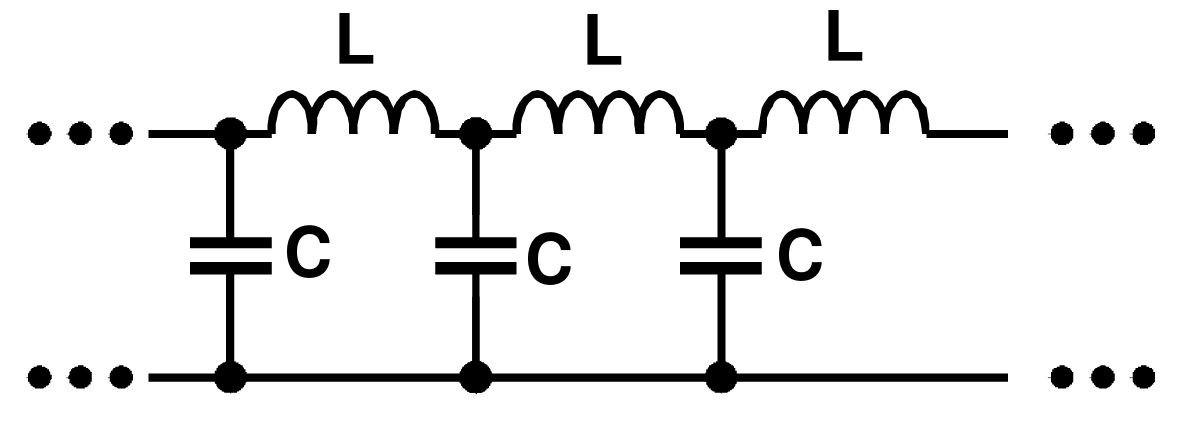
\includegraphics[width=\linewidth-200pt,height=\textheight-200pt,keepaspectratio]{content/Grafiken/LCKette.png}
       \caption{Die unendliche LC-Kette \cite{V356}.}
       \label{fig:LC-Kette}
     \end{figure}

\subsection{Die Eigenschaften einer unendlichen LC-Kette}

Im folgenden wird weiter auf die bereits gennanten Effekte eingegangen. Zunächst
 wird die einfache $LC$-Kette thematisiert. Diese besitzt nur Kondensatoren der
 gleichen Kapazität $C$.\\\\

Aus den kirchhoffschen Regeln folgt die Bewegungsgleichung:
\begin{equation}
- \omega ^2 C U_n + \frac{1}{L} \left( -U_{n-1} + 2U_ n -U{n-1} \right) = 0\text{.}
\end{equation}
Mit einem komplexen e-Ansatz gelangt man zu:
\begin{equation}
 f ^2 = \frac{1}{2LC\pi^2}(1-\cos\theta)
\end{equation}
Dieser Ausdruck wird als Dispersionsrelation bezeichnet und stellt die Frequenz in Abhängigkeit
 der Phasendifferenz pro Kettenglied dar. Anhand der Formel lässt sich erkennen,
  dass der Frequenzbereich indem Schwingungen auftreten begrenzt ist. Daher bilden sich
   für Frequenzen $f \geq \frac{1}{\sqrt{LC\pi^2}}$ keine Schwingungen aus.\\\\

 Nun wird die $LC_1C_2$-Kette näher betracht. Sie besitzt Kondensatoren mit zwei
  verschiedenen Kapazitäten $C_1$ und $C_2$, welche im Wechsel verbaut sind.
 Aus den kirchhoffschen Regeln folgen die Bewegungsgleichungen:
 \begin{equation}
   -\omega^2 C_1 U_{2n+1} + \frac{1}{L} \left( -U_{2n} + 2U_{2n+1} - U_{2n+2} \right) = 0\text{.}
 \end{equation}
 und
 \begin{equation}
   -\omega^2 C_2 U_{2n} + \frac{1}{L} \left( -U_{2n-1} + 2U_{2n+1} - U_{2n+1} \right) = 0\text{.}
 \end{equation}
Es folgt für die auftretende Dispersion:
\begin{equation}
  f_{1/2}^2 = \frac{1}{4\pi^2L}\left(\frac{1}{C_1}+\frac{1}{C_2}\right) \pm \frac{1}{4\pi^2L}\sqrt{\left(\frac{1}{C_1}+\frac{1}{C_2} \right)^2 - \frac{4 \sin^2\theta}{C_1C_2}}\text{.}
\end{equation}
Es zeigt sich, dass die $LC_1C_2$-Kette aufgrund der positiven und negativen Wurzel
zwei Frequenzbereiche besitzt, in denen Schwingungen auftreten. Die Verläufe der
 negativen und postiven Wurzel werden akustischer bzw. optischer Ast genannt.
 Der Kurvenverlauf hat die unten dargestellte Form.
 \begin{figure}[H]
   \centering
   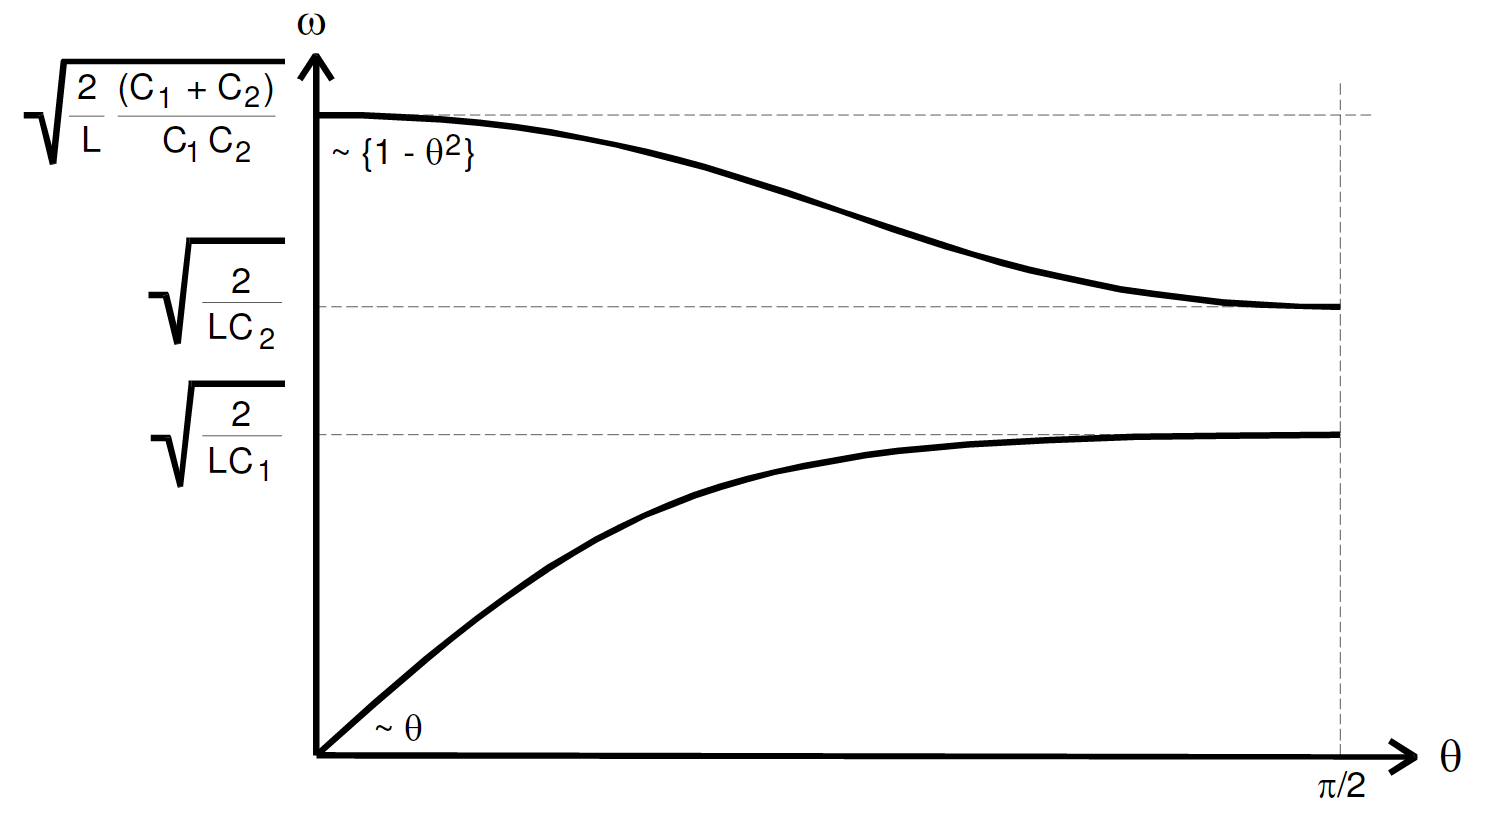
\includegraphics[width=\linewidth-200pt,height=\textheight-200pt,keepaspectratio]{content/Grafiken/Dispersionskurven.png}
   \caption{Die Frequenz in Abhängigkeit der Phasendifferenz \cite{V356}.}
   \label{fig:LC-Kette}
 \end{figure}
 Es zeigt sich, dass zwischen beiden Ästen eine Lücke existiert,
  in denen keine Schwingungen auftreten, da die untere Grenzfrequenz des
   optischen Astes größer ist als die obere Grenzfrequenz des akustischen Astes.


\subsection{Die Eigenschaften einer endlichen LC-Kette}
Liegt eine LC-Kette endlicher Länge vor, bzw. wurden beide Abschlusswiderstände
 nicht nach Formel (1) der Frequenz des Wechselstromes ensprechend angepasst,
  kommt es zur Reflexion ankommender Wellen. Aus den kirchhoffschen Regeln folgt das Verhältnis:
  \begin{equation}
    \frac{U_{ref}}{U_{ein}} = \frac{R-Z}{R+Z}\text{.}
  \end{equation}
  Es folgen die Spezialfälle:\\
\begin{itemize}
  \item Die LC-Kette besitzt ein offenes Ende, $R$ beträgt also $\infty$. An diesem
   wird eine ankommende Welle vollständig und ohne Phasensprung reflektiert.
   Die Phasenunterschiede der entstehenden Bäuche liegen bei Vielfachen von $\pi$.\\

  \item Die LC-Kette ist kurzgeschlossen, $R$ beträgt daher 0. An diesem Ende wird
   eine ankommende Welle vollständig reflektiert, jedoch mit einem Phasensprung von $\pi$.
   Auch hier liegen die Phasenunterschiede der entstehenden Bäuche bei Vielfachen von $\pi$.\\

 \item Werden beide Abschlusswiderstände auf den Wellenwiderstand der LC-Kette eingestellt,
  so verhält sie sich wie eine unendliche LC-Kette. Aus diesem Grund kommt es auch nicht zur Reflexion.
\end{itemize}
